\section{Gestion des Notifications Téléphoniques : Aerogear}

Les notifications sont très importante pour l'application téléphonique Dynamease. En effet ce sont grâce à celles-ci que les informations sur l'appelant sont récupéré par l'appareil. 

\subsection{Fonctionnement des notifications Push}

Une notification est un message envoyé à un smartphone. Ce message à la possibilité de réveiller le smartphone et d'afficher une information. L'envoie d'une notification passe par une plateforme. Pour envoyer une notification à un appareil Android il faut passer par Google Cloud Messaging (GCM). Pour les appareils IOS il faut passer par Apple Push Notification Service (APNS).

Pour cet ensemble de plateforme le fonctionnement est quasiment identique. L'appareil doit s'inscrire à la plateforme correspondante.
Durant cette inscription l'appareil obtient un identifiant unique. Les messages qui lui sont envoyés sont de la forme d'un objet Json (bien que pour Android il soit également possible de passer par un objet de type texte). Les notifications sont utilisés pour envoyer une information à afficher à l'utilisateur (encore une fois pour Android il est également possible d'envoyé une notification pour demander à l'application de se synchroniser sans pour autant afficher de message).

\subsection{Principe d'Aerogear}

Aerogear est une application serveur qui permet l'envoie de notification Push vers différents systèmes d'exploitation téléphonique. En ce qui nous concerne il s'agit d'un envoi vers les systèmes Android et IOS.

L'utilisation de l'API de ce serveur, permet d'envoyer des requêtes vers le serveur Aerogear. Celui-ci aura pour charge de transformer cette requête en une requête adapté pour le système d'exploitation vers lequel la requête doit être envoyée.

Ce procédé permet de délégué l'envoie des notifications Push. Une requête unique permet l'envoie de notification plutôt que d'avoir à effectuer une requête pour chacun des systèmes d'exploitation. De plus le serveur se charge également du stockage des informations des différents systèmes d'exploitation de chaque client.

Les requêtes Aerogear permettent également l'envoie de notification vers toutes les installations, ainsi que l'envoie vers toutes les installation d'un variant spécifique.

\subsubsection{Définitions} 

Avant de décrire le fonctionnement du serveur Aerogear il nous faut définir les différents terme suivant :

\begin{description}
 \item[Application Push :] Représente une application téléphonique ayant recours à des notifications Push.
 \item[Variant :] Représente une plateforme téléphonique comme IOS ou Android. Une application Push peut avoir plusieurs variants. Plusieurs variants peuvent représenter une seule plateforme. Le variant permet de stocker toutes les propriétés nécessaire à l'envoie de notification Push, comme le $"\textit{Google API key}"$ pour Android.
 \item[Installation :] Correspond à une application téléphonique s'étant inscrite sur un variant. Chaque variant peut avoir plusieurs installation. Une installation contient toutes les informations nécessaire à l'envoie de notifications, comme l'id du téléphone.
 \item[Alias :] Correspond à l'identifiant d'une installation.
\end{description}

\subsubsection{Fonctionnement}

\begin{figure}[!h]
	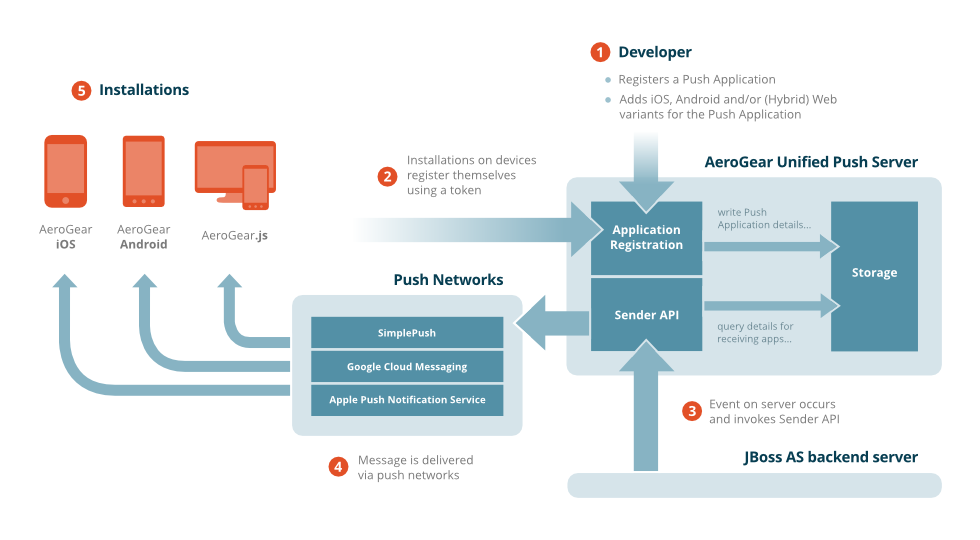
\includegraphics[scale=0.6]{img/aerogear_unified_push_server.png}
	\caption{\label{aerogear} Fonctionnement d'Aerogear}
\end{figure}

Le fonctionnement du serveur Aerogear suit le schéma précédent.

\begin{enumerate}
 \item L'administrateur doit commencer par créé une application Push, qui doit contenir au moins un Variant;
 \item L'application téléphonique demande un enregistrement en envoyant toutes les informations nécessaire à Aerogear. Ces informations sont stockées.
 \item Une requête est envoyé à  Aerogear dans le but d'envoyer une notification vers l'installation correspondant a un alias. Aerogear récupére toutes les informations nécessaire. La requête Push est ensuite traduite vers la plateforme correspondant au système d'exploitation correspondant à l'alias. La requête est ensuite envoyée vers la plateforme appropriée.
 \item C'est maintenant la plateforme qui se charge de l'envoie de la notification vers l'installation correspondant à l'alias.
 \item L'installation reçois la notification, et c'est à l'application téléphonique de gérer le traitement de cette notification.
\end{enumerate}

Les requêtes Aerogear permettent également l'envoie de notification vers toutes les installations, ainsi que l'envoie vers toutes les installation d'un variant spécifique.

\subsection{Mise à jour d'Aerogear}

Mon premier objectif au niveau d'Aerogear était de mettre à jour cette plateforme. Pour ce faire je me suis rendu sur le site officiel afin de connaître les différentes procédure de son installation.

Le serveur Aerogear se présente sous la forme d'un fichier war. Il faut savoir que pour fonctionne, Aerogear à besoin d'un serveur Jboss et d'un base de données. Aerogear peut fonctionner avec différentes base de données SQL (H2, Mysql et postgreSQL). La base utilisée par Dynamease étant une base de données MySQL j'ai donc choisi d'installer la version correspondante.

Plusieurs problème se sont accumulé durant cette installation, en effet des erreurs se produisaient durant le lancement du serveur. Après plusieurs recherche il s'est avéré que le lien donné durant le processus d'installation pointé vers les sources d'une version non stable du projet. Après avoir récupéré un projet stable, j'ai du faire face à une autre difficulté. Le serveur n'arrivait pas à utiliser la base de données MySQL. Après avoir effectué d'autre recherche il a semblait que la version utilisée éprouvé quelques difficultés avec les bases de données MySQL et PostgreSQL, et que seul les base de données de type H2 pouvait être gérées.

Les base de données H2 fonctionnent sous un environnement Java. Afin de pouvoir y accéder de façon graphique le logiciel officiel de cette base de données sera installer également sur le serveur pour pouvoir accédé plus facilement aux données s'y trouvant. Ainsi l'administrateur système pourra aisément réaliser ses requêtes de la même manière qu'il les aurait effectué sur une base de données MySQL.

Après son installation j'ai eu pour objectif de réalisé une Image Docker d'Aerogear. L'explication de cette réalisation sera faîte lors de la partie sur Docker.

\subsection{Mise à jour des notifications}

Après la mise à jour du serveur Aerogear j'ai également dû réaliser des mises à jour du côté des applications téléphonique.

Pour les applications IOS, une mise à jour était nécessaire du fait que certaines méthodes utiles pour l'enregistrement vers le serveur des notifications n'étaient pas rétrocompatible entre la version 7 et la version 8. Comme nous devions garder une version de l'application pour les personnes ayant encore une version IOS7 une vérification de la version de l'appareil est effectué avant tout enregistrement au serveur. Mais il est très probable que l'application Dynamease devienne, dans le futur, inaccessible pour les personnes possédant une version 7 d'IOS. En effet la version 8 permet beaucoup plus de liberté au niveau des notification notamment la possibilité d'ajouter des bouton d'action aux notifications.\\

L'autre mise à jour effectuée est la forme d'envoie des notifications. L'ancienne version envoyé les informations sous la forme de chaîne de caractère. Ces chaînes de caractère était difficile à traité du fait que les informations pouvait être dispersées. La solution la plus évident à mettre en place était de faire passer des objets Json au travers les notifications. En effet, les objets Json sont très facile à créé, à déchiffrer et de plus peuvent être écris sous la forme d'une chaîne de caractère spéciale.

Grâce à cette méthode il est plus facile d'effectuer un traitement sur les informations reçus et de dédier à l'application téléphonique le tri des informations et l'affichage de celle-ci.

\section{L'environnement Docker}
\subsection{Fonctionnement de Docker}
\subsection{Réalisation Docker pour le compte de Dynamease}

\section{Démarrage automatique d'un environnement de travail}

\subsection{Fonctionnalités attendues}

Ce procédé doit permettre aux développeurs de Dynamease de pouvoir mettre en place de façon rapide et automatisé, un environnement de travail complet permettant l'accès aux différents services de Dynamease. 

Il doit également être possible de pré-remplir les bases de données Dynamease, avec des données provenant de base de tests déjà utilisé ou bien d'une base de production.

L'outil ainsi créé devra pouvoir être utilisé aussi bien sur des serveurs que sur les machines locales des développeurs. 

\subsection{Étude du cahier des charges}

Les environnements utilisés par Dynamease peuvent tourner grâce à des container Docker. Pour l'outil qui sera développer, l'utilisation de ces containers sera mise en avant. Il sera donc nécessaire de déterminer l'ordre d'exécution de ces containers, en déterminant les différentes dépendance de ces containers.\\

Il faut également déterminer quels sont les meilleurs solutions pour la mise en place d'un système permettant l'intégration de données au démarrage de l'environnement Dynamease. L'environnement complet de Dynamease est constitué de plusieurs sous environnement, les différents environnement qui nécessitent d'un intégration de données sont :

\begin{itemize}
	\item La base de données MySQL;
	\item La base de données Ldap;
	\item La base de données liée à Aerogear;
	\item Les fichiers de configuration du serveur Dynamease.
\end{itemize}

Il faudra donc déterminer, pour chacun de ces environnement, quels sont les techniques permettant une intégration de données.

De plus il doit être possible de démarrer d'un environnement vide, il faudra donc gérer ce cas de figure, en initialisant les bases de données de manière à ce qu'elles soient utilisable dans l'environnement complet de Dynamease.

\subsection{Réalisation de l'outil}

\subsubsection{Détermination des dépendances}

[Mettre Diagramme pyramide]

Nous allons étudier le diagramme ci-dessus, de manière descendante. Tout en haut nous avons l'environnement Nginx, celui-ci nécessite la mise en place des environnements Tomcat et Aerogear pour fonctionner. L'environnement Tomcat nécessite l'existence des bases de données MySQL et Ldap. 

Donc il nous faudra lancer l'environnement l'ordre suivant :

\begin{enumerate}
	\item La base de données MySQL;
	\item La base de données Ldap;
	\item Aerogear;
	\item Tomcat;
	\item Nginx.
\end{enumerate}

\subsubsection{Récupération et utilisation des données}

Le fonctionnement de l'environnement Dynamease dépend de plusieurs données, on doit donc récupérer ces données. On peut séparer les données à récupérer en deux catégories, les données de configuration et les données de stockage d'informations.

Les données récupérées, par le serveur Tomcat de Dynamease, sont essentiellement des données de configuration. Cette configuration permet à Dynamease de connaître les adresses internet des différents services nécessaire à son fonctionnement. Ces adresses peuvent être différentes d'un environnement à un autre selon l'emplacement de démarrage de l'application Dynamease. Le mieux est donc d'avoir ces fichiers stockés sur l'emplacement de démarrage.

Pour ce type de données, il sera demandé la création d'une variable d'environnement par l'utilisateur afin de lui permettre de préciser à l'outil, l'emplacement des différents fichiers de configuration de Dynamease. 

Des fichiers de configurations par défaut seront présent dans l'outil. Si l'utilisateur ne désigne pas de répertoire contenant ces fichiers de configurations, un message sera affiché pour le prévenir que les fichiers de configuration par défaut seront utilisés, mais que cela peut entraîner quelques dysfonctionnement.\\

En ce qui concerne les données des différentes bases de données, celles-ci peuvent être stockées indépendamment de leur bases de données d'origine. Seul leur intégration sera différente.

Il nous reste donc trois base de données à remplir avec nos fichiers de données. Leur technique d'intégration étant différente nous allons les étudier pour chaque base de données. 

[Explication schéma ?] 

Deux solutions de stockage peuvent être étudiés, on pourrait utiliser les volumes de chaque containers, en intégrant les données. Cette méthode risque d'être assez limité sachant que chaque utilisateur devra disposer des fichiers de données afin de les intégrer dans son environnement. La seconde solution serait d'utiliser une nouvelle image Docker qui aura pour rôle le stockage de tout les fichiers de données. Cette solution permettrait de pouvoir utiliser n'importe quelle base de donné sans récupérer les fichiers de données. C'est cette seconde solution que nous allons développer par la suite.

Cette solution prend en compte que le container de données contienne des volumes pour stocker les fichiers de données. Or, comme nous l'avons vu précédemment, les volumes créés des liens symboliques depuis les volumes du container vers les répertoires situés sur la machine faisant tourner le container. Donc le container serait opérationnel uniquement sur la machine l'ayant créé, si ce container se trouve sur un autre système, il se peut que les liens ne pointes sur aucuns fichiers ou sur de mauvais fichiers. 

On a également vu qu'on pouvait exécuter des commandes lors de la création du container. L'idée est d'utiliser un script de démarrage du container, qui nous servira à déplacer et trier les fichiers de données vers de nouveaux répertoires.

Grâce à cette récupération nous pouvons maintenant faire un traitement pour chaque fichier selon le type de base de données où celui-ci doit être inclue.\\

Il est aussi prévu de permettre aux utilisateurs de cet outil de lancer un environnement de travail, vide. C'est à dire seulement avec les bases de données initialisées, mais sans données. Pour cela l'image du docker de stockage des données sera généré avec les fichiers d'initialisation de chacune des bases de données. Un script de démarrage aura pour rôle de déterminer si des fichiers d'intégration de données sont présente, si c'est le cas, ces fichiers seront déplacé vers le répertoire correspondant à la base de données, sinon se seront les fichiers d'initialisation qui y seront placés. 

\subsubsection{Récupération de la version Dynamease}

Le lancement de l'environnement de travail Dynamease, doit être précisé d'un numéro de version du serveur Dynamease. 

Chaque version de Dynamease est présent sur le \textit{repository} Docker de Dynamease. Chaque nouvelle version déposé sur le serveur Git est récupérée par le serveur Jenkins. Celui-ci aura pour charge de vérifier le bon fonctionnement de la version déposée. Si celle-ci est correcte alors une nouvelle image Docker du serveur est créée avec le nom du commit comme numéro de version.

La création d'une image docker Dynamease, nécessite d'abord la compilation de l'ensemble du code source de Dynamease, de la récupération des archives (war) du serveur et enfin de leur intégration vers la nouvelle image Docker.

Le script de démarrage de l'environnement prendra en paramètre un numéro de version. Il vérifiera alors si l'image est présente en local, si ce n'est pas le cas l'image sera télécharger depuis le serveur Docker.

Grâce à cette méthode, il est possible de démarrer rapidement n'importe quel version de Dynamease.

\section{Outils d'aide à la mesure des performances}

\section{Amélioration des applications téléphoniques}

Nous allons maintenant aborder les différentes améliorations que nous devions réaliser après la réalisation de plusieurs tests de performance.

\subsection{Récupération des contacts Ios}

En début de stage un problème nous a été reporté par un utilisateur de l'application Iphone. L'application ne démarrer pas sur son Iphone. En effet tout de suite après la connexion de l'utilisateur, l'application se fermer subitement. Nous avons donc tenter de reproduire ce dysfonctionnement sur nos téléphone de test. Pourtant il nous était impossible de déterminer d'où venait l'erreur.

Nous avons donc demander le modèle d'Iphone et la version IOS de l'Iphone afin de pouvoir reproduire la procédure d'erreur dans les mêmes conditions. Mais encore une fois l'application semblait très bien fonctionner sur nos téléphone de test. Nous avons également demander à l'utilisateur de se connecter à l'aide d'un de nos téléphone de test, mais l'erreur ne s'est pas reproduite.

Nous en avons donc conclu que l'erreur devait provenir d'une configuration spéciale de l'Iphone de l'utilisateur.

Nous avons donc lister les différentes méthodes exécutée par l'application au démarrage, afin de déterminer celle qui aurait pu interagir directement avec une configuration spéciale de l'utilisateur.

[Diagramme de Mise en service de l'application]

Les différentes méthodes exécuter par l'application étaient, la récupération des informations de l'utilisateur auprès du serveur Dynamease, la récupération des contacts du portable et l'inscription sur le serveur Aerogear.

Après une observation sur les logs des serveurs Dynamease et Aerogear, nous nous sommes aperçus que les données de l'utilisateur été bien envoyé mais que le serveur Aerogear ne recevait pas de requête d'inscription.

L'erreur provenait donc de la récupération des contacts. De plus nous avons remarquer que l'utilisateur avait énormément de contact. Le problème pouvait donc provenir soit d'un contact particulier de l'utilisateur dont les informations étaient mal traitées, ou bien que le nombre important de contact faisait fermer subitement l'application.

Pour éviter de demander la liste de contacts de l'utilisateur nous avons décider en premier lieu de se pencher sur la seconde solution en créant des centaines de contact que nous importerions par la suite dans le téléphone de test. L'application arriva parfaitement à traiter ces centaines de contact.

Nous avons donc du demander la liste de contact de l'utilisateur dans le but de détecter quel était le contact qui produisait cette erreur, et quelle était la cause.

Après l'importation de ces contacts, nous avons remarqué que l'erreur se produisait également  sur les téléphones de tests. Après une observation des logs généré par l'application il est apparu qu'il existait un contact dont le nom commencé par le caractère $'@'$.

Les contacts dans l'application Iphone sont stocké dans un dictionnaire (ensemble clefs valeurs). Les clefs sont représenté par le noms de l'utilisateur et les valeurs sont les informations relative à l'utilisateur. La clef est donc de type chaîne de caractère. Or en Objective-C le caractère $'@'$ est un caractère spécial. L'Iphone n'arrivant pas à interpréter ce caractère l'application ferma subitement.

Afin de régler ce type de problème, un caractère spécial $'\textbackslash'$ est ajouté devant chaque caractère spécial pouvant être trouvé dans le nom ou les informations clients. Ce caractère à pour fonction, dans l'Objective-C de signifier à l'application de ne pas interpréter le caractère spécial qui le suit. 

\subsection{Recherche et récupération automatique des contacts}


\subsubsection{Recherche de contact}

L'application Téléphonique Android, permet aux utilisateurs d'avoir une liste de contact. Cette liste de contact est triée par défaut dans l'ordre alphabétique par rapport aux noms de famille des contacts. De plus une barre de recherche est disponible pour faire une recherche dans cette liste.

La version précédent ma correction, n'effectuait la recherche uniquement sur le nom, de plus sur de longue liste de contact, la recherche pouvait prendre beaucoup de temps.

La première étape pour effectuer une correction est d'observer la technique utilisait pour cette recherche, ainsi que les différents procédés utilisés par la liste de contact.\\\\



En premier lieu j'ai étudié les différents moyens de stockage que proposait Android. Celle-ci propose trois moyens de stockage qui sont :

\begin{enumerate}
	\item Stockage par le biais de clef valeur;
	\item Stockage dans un fichier texte;
	\item Stockage à l'aide d'une base de données SQL Light.
\end{enumerate}

La première technique peut être utilisée pour de petites valeurs uniques, comme le nom de l'utilisateur, son numéro de téléphone, etc.

Le fichier texte est surtout utilisé si on doit générer des fichiers de données, pouvant être récupéré par l'utilisateur.

La base de données SQL est utilisé pour stocker des liste de données suivant le même schéma.

C'est cette dernière option qui nous intéresse pour le stockage de la liste de contact. C'est effective cette technique de stockage qui est utilisée pour le stockage des contacts.

Un contact normal est représenté par son nom, son prénom, son numéro de téléphone. Un contact Dynamease est représenté par son nom, son prénom et son Id Dynamease. C'est deux type de contact son stocké dans la même table de données, et son différencié par une variable booléenne qui est à vrai si le contact est un contact Dynamease et est à faux sinon.\\\\

L'algorithme anciennement utilisé pour la recherche des contacts suivait le diagramme suivant :

[Mettre diagramme]

A chaque fois que l'utilisateur entre une lettre dans la barre de recherche, le processus de la recherche est lancé. Pour chaque contact de la liste, on vérifie si l'ensemble des lettres, entrées dans la barre de recherche, est présent dans le nom du contact. Si on trouve une correspondance entre l'ensemble des lettres et le nom du contact on ajoute ce contact à la liste de retour. Et on effectue cette correspondance pour chaque contact.

Ce processus est long en raison la recherche sur toute la liste de contact à chaque ajout de lettre dans la barre de recherche. L'autre problème flagrant est que la recherche n'est effectué que sur le nom.\\\\

La première résolution de ce problème suit le processus suivant :

[Mettre Diagramme]

Avant toute recherche la liste de contact est contenu dans le résultat à retourner. Par défaut tout les contacts correspondent à une recherche vide. A chaque ajout de lettre, on recherche dans la liste dernièrement retournée les contacts ayant l'ensemble des lettres de recherche dans leur prénom ou dans leur nom. Si une correspondance est trouvé alors le contact est ajouté dans une liste temporaire. Une fois tous les contacts vérifiés, on remplace la liste de résultat par la liste temporaire, et on renvoie la liste de résultat. Et on continue sur le même principe à chaque ajout de lettre\\\\

Le problème de cette solution c'est que l'ordre des mots de recherche est importante faire une recherche $"\textit{nom prénom}"$ ne sera pas interprété de la même façon que la recherche $"\textit{prénom nom}"$.

[Mettre diagramme]

On reprend le même principe que précédemment, mais cette fois-ci on fait un travail supplémentaire entre l'ajout d'une lettre et la recherche dans la liste de contact. On sépare les différents mots de la barre de recherche. Pour la estime qu'il y a un nouveau mot à chaque fois que la barre espace est pressée. Ensuite la recherche dans les contacts doit correspondre à chaque mot de la barre de recherche. Si un mot ne correspond pas, alors le contact ne sera pas ajouter à la liste de résultat. Tous les mots doivent correspondre, pour que le contact soit ajouter dan la liste de résultat.

\subsubsection{Récupération des contacts du téléphone}

La récupération des contacts ne semblait s'effectuer qu'une seule fois, lors du premier lancement de l'application. De plus il existait quelques problème au niveau du temps de récupération des contacts. Plus la liste de contact était grande et plus le temps de récupération était longue (par exemple pour une liste de contact de 10000 contacts le chargement pouvait être de quelques jours).\\

Après une inspection du code, l'activité de la liste de contact se chargé de la récupération des contacts à chaque lancement de cette activité. Or cette récupération avait une mauvaise condition pour la récupération des contacts.

La liste de contact est stockée par ordre alphabétique dans la base de données de Dynamease, c'est également le cas pour la liste de contact du téléphone. L'activité vérifie que le nombre de contacts dans la liste de contact du téléphone est égale au nombre de contact de la liste de contact de l'application Dynamease. Si ce n'est pas le cas une vérification est effectuée. Le problème se situe sur la suite du procédé. Le cursor permettant la récupération est programmer pour récupérer les contacts en partant de l'index correspondant au nombre de contact dans la liste de contact Dynamease moins un. Or les contacts stockés dans la base de données du téléphone ne sont pas trié par ordre chronologique mais par ordre alphabétique. Donc si un contact, ajouté à la suite du premier démarrage, est ajouté au début de la liste de contact, alors il ne sera jamais récupéré, et le programme fera une récupération de contact à chaque démarrage de l'activité.

La recherche est maintenant effectuée sur l'ensemble de la liste de contact du téléphone est une vérification sur l'existence des contacts est également effectuée, afin de ne pas avoir de doublon.\\ 

La récupération des contacts s'effectue par des \textit{Task}. Comme un \textit{Thread}, plusieurs \textit{Task} peuvent être en fonction "simultanément". Donc à chaque fois que l'activité de la liste de contact est lancée, la \textit{Task} de récupération des contacts est lancé. Donc le temps processeur est divisé entre ces deux \textit{Task}. Pour améliorer cette récupération une condition est rajouter pour déterminer si une récupération est déjà en cour afin de ne pas re-diviser le temps processeur. De plus un bouton d'actualisation de la liste de contact a été ajouter. Dorénavant, la récupération des contacts s'effectue seulement si la liste de contact de l'application Dynamease est vide ou si l'utilisateur appuie sur le bouton d'actualisation.

\subsubsection{Récupération des images de profile}

Il est apparu également qu'à chaque affichage de la liste de contact, dans l'application Android, une requête pour récupérer les images de profiles Dynamease est envoyé. Ces requêtes n'ont pas forcément lieu d'être effectuées à chaque affichage. En effet, le changement d'image de profile est beaucoup trop rare pour qu'une requête soit envoyé aussi couramment.

La requête de récupération des images s'effectue grâce à une requête Json. Le résultat de la requête se présente sous la forme d'une suite de caractère représentant l'image. Cette récupération est effectuée pour l'affichage des images dans la liste de contact. Il faut donc trouver une solution pour ne pas avoir à effectuer une requête pour l'affichage des images.

Le plus simple est de stocker les images sur l'appareil de l'utilisateur. Nous avons exploré précédemment les différentes techniques de stockages qu'offrait Android. La meilleure solution est d'utiliser l'écriture de fichier. Ce type de stockage, effectue, par défaut, la sauvegarde dans un dossier spécifique à l'application.On récupérera donc la suite de caractère pour la stocker dans un fichier. 

La récupération des images doit au moins être effectué une fois. Pour cela on suivra l'algorithme suivant :

[mettre Diagramme]

Lors de l'affichage de la liste de contact, à chaque contact Dynamease on fait la vérification suivante. On vérifie si l'image de profile est présente dans le répertoire de l'application Dynamease. Si l'image n'est pas présente, on envoie une requête vers le serveur Dynamease, afin de la récupérer. Une fois cette image récupérée, on stocke la suite de caractère récupérée dans un fichier. Le fichier de sorti aura sera nommé comme l'Id Dynamease du contact.

Ainsi l'affichage des images se fera par le biais de la récupération des fichiers images présent sur l'appareil téléphonique.

\subsubsection{Amélioration possible}

La récupération des images ne se fait qu'une seule fois. Or il est possible qu'un contact change son image de profile. Aucune mise à jour ne sera effectuée avec la méthode actuelle. Il faut donc penser à une solution pour que les images de profiles soient mises à jours. Pour cela on pourrait utiliser le bouton de rafraîchissement de contact déjà utilisé pour mettre la liste des contacts du téléphone à jour. 
